\documentclass[11pt,oneside,leqno]{article}
\usepackage[paperwidth=6.5in,paperheight=9.5in,margin=.72in]{geometry}
\usepackage{fontspec}
\setmainfont{lmroman10-regular.otf}[BoldFont=lmroman10-bold.otf,ItalicFont=lmroman10-italic.otf,BoldItalicFont=lmroman10-bolditalic.otf,SmallCapsFont=lmromancaps10-regular.otf]
\usepackage{amsmath,amssymb,graphicx,tikz,microtype,needspace}
\usepackage[unicode,hidelinks]{hyperref}
\hypersetup{pdftitle={Weitere Fragmente über das Pentagramma mirificum},pdfauthor={Carl Friedrich Gauss}}
\newcommand{\SourceLeaf}[1]{\hypertarget{native-#1}{}}
\newcommand{\BareRoot}[1]{\mathord{\surd}#1}
\renewcommand{\thefootnote}{*)}
\setlength{\parindent}{1.2em}
\setlength{\emergencystretch}{1.4em}
\widowpenalty=10000\clubpenalty=10000\raggedbottom
\newcommand{\StepDown}[2]{\raisebox{-#1em}{$\displaystyle #2$}}
\newcommand{\TriLetter}[1]{\tikz[baseline=-.55ex,x=1ex,y=1ex,line width=.35pt]{\draw (0,0)--(2.1,2.1)--(4.2,0)--cycle;\node[inner sep=0pt] at (2.1,.65) {$\scriptstyle #1$};}}
\newcommand{\Arc}[1]{\overset{\frown}{#1}}
\newcommand{\HistAngle}{\mathord{\tikz[baseline=-.3ex,x=1ex,y=1ex,line width=.35pt]{\draw (1.35,1.0)--(0,.5)--(1.35,0);\draw (.18,1.18) .. controls (.85,.95) and (.85,.05) .. (.18,-.18);}}}
\begin{document}
\SourceLeaf{113}

\begin{center}\textbf{[WEITERE FRAGMENTE ÜBER DAS PENTAGRAMMA MIRIFICUM.]}\end{center}

\begin{center}\rule{1.5cm}{.4pt}\end{center}

\begin{center}[9.]\end{center}

Die Exponenten der Verjüngung der Hauptaxen der centralen Projectionsellipse sind:

\[
\sqrt{\dfrac{G'-1}{G'}} = \dfrac{2G'-1}{\sqrt{\alpha\beta\gamma\delta\varepsilon}} \quad \text{für die erste Axe } \dfrac{1}{\sqrt{G'}},
\]
\[
\sqrt{\dfrac{G''-1}{G''}} = \dfrac{2G''-1}{\sqrt{\alpha\beta\gamma\delta\varepsilon}} \quad \text{für die zweite Axe } \dfrac{1}{\sqrt{G''}},
\]
oder weil

\[
GG'G'' = -\tfrac14 \alpha\beta\gamma\delta\varepsilon,
\]
\[
(G-1)(G'-1)(G''-1) = -\tfrac14,
\]
\[
(2G-1)(2G'-1)(2G''-1) = -\alpha\beta\gamma\delta\varepsilon
\]
[gilt], die Verjüngung der projicirten Axen $= \dfrac{1}{1-2G}$.

Es ist vortheilhaft, neben den vorigen Grössen $G$, $G'$, $G''$ auch die Wurzeln der Gleichung:

\[
\frac{u^3+u}{uu-1} = \sqrt{\alpha\beta\gamma\delta\varepsilon}
\]
einzuführen. Sind dieselben $\xi$, $\eta$, $\zeta$, so ist:

\[
\xi+\eta+\zeta = -\xi\eta\zeta = \sqrt{\alpha\beta\gamma\delta\varepsilon},
\]
\[
\xi\eta+\eta\zeta+\zeta\xi = 1,
\]

\SourceLeaf{114}
\[
G = \frac{\zeta\zeta}{\zeta\zeta-1} \quad \text{oder} \quad \zeta = \sqrt{\frac{G}{G-1}},
\]
\[
G' = \frac{\xi\xi}{\xi\xi-1} \quad \text{oder} \quad \xi = \sqrt{\frac{G'}{G'-1}},
\]
\[
G'' = \frac{\eta\eta}{\eta\eta-1} \quad \text{oder} \quad \eta = \sqrt{\frac{G''}{G''-1}}.
\]

\Needspace{8\baselineskip}Auf das innere Pentagon (das sphärische) beziehen sich die Coordinaten:

\[
\frac{\dfrac{x}{\xi}}{\sqrt{\dfrac{xx}{\xi\xi}+\dfrac{yy}{\eta\eta}+\dfrac{zz}{\zeta\zeta}}}, \quad
\frac{\dfrac{y}{\eta}}{\sqrt{\dfrac{xx}{\xi\xi}+\dfrac{yy}{\eta\eta}+\dfrac{zz}{\zeta\zeta}}}, \quad
\frac{\dfrac{z}{\zeta}}{\sqrt{\dfrac{xx}{\xi\xi}+\dfrac{yy}{\eta\eta}+\dfrac{zz}{\zeta\zeta}}};
\]
auf das folgende innere würde sich beziehen:

\[
\frac{\dfrac{x}{\xi\xi}}{\sqrt{\dfrac{xx}{\xi^4}+\dfrac{yy}{\eta^4}+\dfrac{zz}{\zeta^4}}}, \quad
\frac{\dfrac{y}{\eta\eta}}{\sqrt{\dfrac{xx}{\xi^4}+\dfrac{yy}{\eta^4}+\dfrac{zz}{\zeta^4}}}, \quad
\frac{\dfrac{z}{\zeta\zeta}}{\sqrt{\dfrac{xx}{\xi^4}+\dfrac{yy}{\eta^4}+\dfrac{zz}{\zeta^4}}}
\]
u.\,s.\,f. Für das äussere hingegen sind die Coordinaten:

\[
\frac{\xi x}{\sqrt{\xi\xi xx+\eta\eta yy+\zeta\zeta zz}}, \quad
\frac{\eta y}{\sqrt{\xi\xi xx+\eta\eta yy+\zeta\zeta zz}}, \quad
\frac{\zeta z}{\sqrt{\xi\xi xx+\eta\eta yy+\zeta\zeta zz}},
\]
u.\,s.\,f.

Für unser Beispiel, wo $\alpha\beta\gamma\delta\varepsilon = 20$ ist, sind die Zahlwerthe:

\[
\xi = 3{,}9276268 \qquad \eta = 1{,}3735071 \qquad \zeta = -0{,}8289980.
\]

\begin{center}\rule{3cm}{.4pt}\end{center}

\Needspace{12\baselineskip}\begin{center}[10.]\end{center}

$\lambda$, $\mu$ Verjüngungscoefficienten (negative Brüche).

\[
\begin{aligned}
a,\; a\lambda,\; a\lambda\lambda,\; a\lambda^3,\; \ldots \\
b,\; b\mu,\; b\mu\mu,\; b\mu^3,\; \ldots
\end{aligned}
\Bigg\} \begin{gathered}\text{successive Hauptaxen}\\\text{der Projectionsellipsen.}\end{gathered}
\]

$a\xi+b\eta i$, $a\xi'+b\eta' i$ u.\,s.\,w. die fünf Polygonpunkte (in Sternform).

$\lambda$, $\mu$, $\nu$ Wurzeln der Gleichung

\[
\frac{\lambda\lambda+1}{\lambda^3-\lambda} = \frac{\mu\mu+1}{\mu^3-\mu} = \frac{\nu\nu+1}{\nu^3-\nu} = \sqrt{\alpha\beta\gamma\delta\varepsilon} = \frac{1}{\omega}.
\]

\SourceLeaf{115}

\[
\lambda+\mu+\nu=\lambda\mu\nu=\omega,
\]
\[
\lambda\mu+\mu\nu+\nu\lambda+1=0,
\]
\[
\lambda\lambda+\mu\mu+\nu\nu=\omega\omega+2.
\]
\[
\lambda=\operatorname{tang}\boldsymbol{L}, \qquad \mu=\operatorname{tang}\boldsymbol{M}, \qquad \nu=\operatorname{tang}\boldsymbol{N},
\]
\[
\boldsymbol{L}+\boldsymbol{M}+\boldsymbol{N}=0.
\]

In unserm Beispiele:
\[
\boldsymbol{L}=-14^{0}17'4'', \qquad \boldsymbol{M}=-36^{0}3'26'', \qquad \boldsymbol{N}=50^{0}20'30''.
\]
\[
G'=\frac{1}{1-\lambda\lambda}=\frac{\cos \boldsymbol{L}^{2}}{\cos 2\boldsymbol{L}},
\]
\[
G''=\frac{1}{1-\mu\mu}=\frac{\cos \boldsymbol{M}^{2}}{\cos 2\boldsymbol{M}},
\]
\[
G\phantom{'}=\frac{1}{1-\nu\nu}=\frac{\cos \boldsymbol{N}^{2}}{\cos 2\boldsymbol{N}},
\]
\[
(1-\lambda\lambda)\xi\xi'+(1-\mu\mu)\eta\eta'+(1-\nu\nu)=0,
\]
\[
\left(\lambda+\frac{1}{\lambda}\right)\xi\xi'+\left(\mu+\frac{1}{\mu}\right)\eta\eta'+\left(\nu+\frac{1}{\nu}\right)=0,
\]
\[
\left(\lambda-\frac{1}{\lambda}\right)\xi\xi''+\left(\mu-\frac{1}{\mu}\right)\eta\eta''+\left(\nu-\frac{1}{\nu}\right)=0,
\]
\[
\frac{\lambda\lambda+1}{\lambda\lambda}\,\xi\xi''+\frac{\mu\mu+1}{\mu\mu}\,\eta\eta''+\frac{\nu\nu+1}{\nu\nu}=0,
\]
\[
\frac{\xi\xi'}{\sin 2\boldsymbol{L}}+\frac{\eta\eta'}{\sin 2\boldsymbol{M}}+\frac{1}{\sin 2\boldsymbol{N}}=0,
\]
\[
\frac{\xi\xi''}{\operatorname{tang} 2\boldsymbol{L}}+\frac{\eta\eta''}{\operatorname{tang} 2\boldsymbol{M}}+\frac{1}{\operatorname{tang} 2\boldsymbol{N}}=0.
\]

Die vier Punkte $\lambda\xi+\mu\eta i$, $\xi'+\eta'i$, $\xi''+\eta''i$, $\lambda\xi'''+\mu\eta'''i$ liegen in einer geraden
Linie, und ebenso vier andere Combinationen von je vier anderen Punkten.

\[
\frac{\lambda\lambda+1}{\lambda}(\xi'''-\xi)\xi''''=\frac{\mu\mu+1}{\mu}(\eta-\eta''')\eta'''',
\]
\[
\frac{\lambda\lambda+1}{\lambda\lambda}(\xi'-\xi'')\xi''''=\frac{\mu\mu+1}{\mu\mu}(\eta''-\eta')\eta''''.
\]

\begin{center}\rule{3cm}{.4pt}\end{center}

\SourceLeaf{116}

\clearpage\begin{center}[11.]\end{center}

\noindent\begin{minipage}[t]{.46\textwidth}
\vspace{0pt}
\[
\begin{gathered}
\beta+\varepsilon+\lambda=\boldsymbol{A}, \\
\gamma+\alpha+\lambda=\boldsymbol{B}, \\
\delta+\beta+\lambda=\boldsymbol{C}, \\
\varepsilon+\gamma+\lambda=\boldsymbol{D}, \\
\alpha+\delta+\lambda=\boldsymbol{E},
\end{gathered}
\]

\[
\begin{gathered}
\gamma+\delta+\lambda=\boldsymbol{A}', \\
\delta+\varepsilon+\lambda=\boldsymbol{B}', \\
\varepsilon+\alpha+\lambda=\boldsymbol{C}', \\
\alpha+\beta+\lambda=\boldsymbol{D}', \\
\beta+\gamma+\lambda=\boldsymbol{E}',
\end{gathered}
\]

\end{minipage}\hfill\begin{minipage}[t]{.50\textwidth}
\vspace{0pt}
\begin{center}\resizebox{5.1cm}{!}{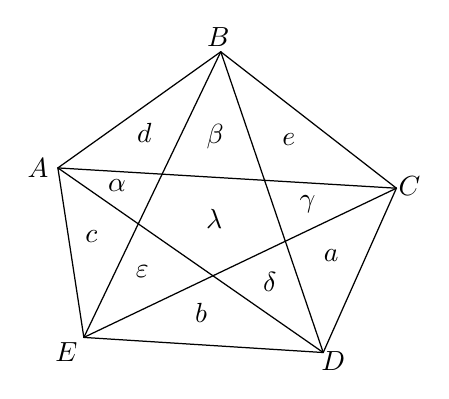
\begin{tikzpicture}[x=.006cm,y=-.006cm,line width=.45pt,line cap=round,line join=round,every node/.style={inner sep=0pt,font=\normalsize}]
\coordinate (A) at (177,347);
\coordinate (B) at (522,101);
\coordinate (C) at (894,390);
\coordinate (D) at (739,738);
\coordinate (E) at (232,706);
\draw (A) -- (B);
\draw (B) -- (C);
\draw (C) -- (D);
\draw (D) -- (E);
\draw (E) -- (A);
\draw (A) -- (C);
\draw (A) -- (D);
\draw (B) -- (E);
\draw (B) -- (D);
\draw (C) -- (E);
\node at (135,347) {$A$};
\node at (517,70) {$B$};
\node at (922,385) {$C$};
\node at (760,756) {$D$};
\node at (195,738) {$E$};
\node at (360,272) {$d$};
\node at (510,280) {$\beta$};
\node at (666,286) {$e$};
\node at (302,384) {$\alpha$};
\node at (706,424) {$\gamma$};
\node at (508,456) {$\lambda$};
\node at (248,493) {$c$};
\node at (356,566) {$\varepsilon$};
\node at (756,533) {$a$};
\node at (626,588) {$\delta$};
\node at (480,655) {$b$};
\end{tikzpicture}
}\end{center}

\[
\begin{gathered}
c+d+\alpha=\mathfrak{A}, \\
d+e+\beta=\mathfrak{B}, \\
e+a+\gamma=\mathfrak{C}, \\
a+b+\delta=\mathfrak{D}, \\
b+c+\varepsilon=\mathfrak{E},
\end{gathered}
\]
\end{minipage}


\[
a+b+c+d+e=s,
\]
\[
\alpha+\beta+\gamma+\delta+\varepsilon=\sigma,
\]
\[
\boldsymbol{A}+\boldsymbol{B}+\boldsymbol{C}+\boldsymbol{D}+\boldsymbol{E}=\boldsymbol{S}=\boldsymbol{A}'+\boldsymbol{B}'+\boldsymbol{C}'+\boldsymbol{D}'+\boldsymbol{E}',
\]
\[
\mathfrak{A}+\mathfrak{B}+\mathfrak{C}+\mathfrak{D}+\mathfrak{E}=\mathfrak{S},
\]
\[
\boldsymbol{S}=2\sigma+5\lambda=\boldsymbol{S}',
\]
\[
\mathfrak{S}=\sigma+2s, \qquad \omega=s+\sigma+\lambda.
\]

Proportionalitäten:
\[
a\boldsymbol{A}=(e+\gamma)(b+\delta),
\]
\[
b\boldsymbol{B}=(a+\delta)(c+\varepsilon),
\]
\[
c\boldsymbol{C}=(b+\varepsilon)(d+\alpha),
\]
\[
d\boldsymbol{D}=(c+\alpha)(e+\beta),
\]
\[
e\boldsymbol{E}=(d+\beta)(a+\gamma),
\]

\SourceLeaf{117}
alle aus dem Princip, dass die Producte aus den von einander abgekehrten (bloss
gemeinschaftliche Spitze habenden, oder noch concinner, keine gemeinschaftliche Seite
habenden) Dreiecken, in welche ein Viereck durch die Diagonalen zerlegt wird, gleich sind.

Die allgemeine barycentrische Gleichung zwischen vier Punkten, z.\,B. $(A)$, $(B)$, $(C)$,
$(D)$ ist:
\[
\TriLetter{A}\,(A)+\TriLetter{B}\,(B)+\TriLetter{C}\,(C)+\TriLetter{D}\,(D)=0,
\]
wo $\TriLetter{A}$ das Dreieck $BCD$, $\TriLetter{B}$ das Dreieck $CDA$
u.\,s.\,w. (mit Rücksicht auf [das] Zeichen) vorstellt. In unserm Fall wird, wenn man zu
obigen Bezeichnungen noch setzt:
\[
\boldsymbol{A}^{*}=\alpha+\gamma+\delta+a+\lambda, \quad \text{u.\,s.\,w.}
\]
\[
\boldsymbol{A}^{*}=\omega-\mathfrak{B}-\mathfrak{E}, \quad \text{u.\,s.\,w.},
\]
der Typus der Gleichung zwischen vier Punkten:
\[
\mathfrak{C}(A)+\boldsymbol{D}^{*}(C)=\boldsymbol{A}^{*}(B)+\mathfrak{B}(D),
\]
wo $(A)$ den betreffenden Eckpunkt des äussern Pentagons ausdrückt, oder:
\[
\begin{gathered}\mathfrak{C}(A)+(\omega-\mathfrak{E}-\mathfrak{C})(C)\\=(\omega-\mathfrak{B}-\mathfrak{E})(B)+\mathfrak{B}(D)\\=(\omega-\mathfrak{E})(e),\end{gathered}
\]
wo $(e)$ den betreffenden Punkt des inneren Pentagons ausdrückt.

\begin{center}\rule{3cm}{.4pt}\end{center}

\begin{center}\resizebox{7cm}{!}{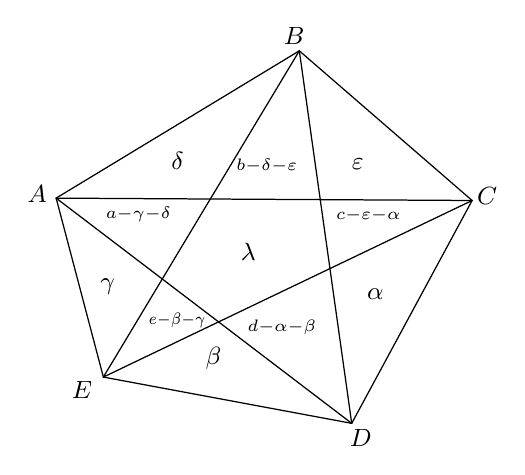
\begin{tikzpicture}[x=.006cm,y=-.006cm,line width=.45pt,line cap=round,line join=round,every node/.style={inner sep=0pt,font=\small}]
\coordinate (A) at (158,408);
\coordinate (B) at (673,96);
\coordinate (C) at (1039,413);
\coordinate (D) at (784,885);
\coordinate (E) at (258,787);
\draw (A) -- (B);
\draw (B) -- (C);
\draw (C) -- (D);
\draw (D) -- (E);
\draw (E) -- (A);
\draw (A) -- (C);
\draw (A) -- (D);
\draw (B) -- (E);
\draw (B) -- (D);
\draw (C) -- (E);
\node at (118,400) {$A$};
\node at (662,65) {$B$};
\node at (1071,403) {$C$};
\node at (803,916) {$D$};
\node at (213,814) {$E$};
\node at (415,330) {$\delta$};
\node at (604,339) {$\scriptstyle b-\delta-\varepsilon$};
\node at (797,337) {$\varepsilon$};
\node at (332,443) {$\scriptstyle a-\gamma-\delta$};
\node at (819,445) {$\scriptstyle c-\varepsilon-\alpha$};
\node at (565,522) {$\lambda$};
\node at (267,596) {$\gamma$};
\node at (414,666) {\scalebox{.86}[1]{$\scriptstyle e-\beta-\gamma$}};
\node at (491,747) {$\beta$};
\node at (636,681) {$\scriptstyle d-\alpha-\beta$};
\node at (834,612) {$\alpha$};
\end{tikzpicture}
}\end{center}

\[
\boldsymbol{A}c\varepsilon+\boldsymbol{C}c(b-\varepsilon)=\boldsymbol{B}b(c-\varepsilon)+\boldsymbol{D}b\varepsilon,
\]
\[
\boldsymbol{B}d\alpha+\boldsymbol{D}d(c-\alpha)=\boldsymbol{C}c(d-\alpha)+\boldsymbol{E}c\alpha,
\]
\[
\boldsymbol{C}e\beta+\boldsymbol{E}e(d-\beta)=\boldsymbol{D}d(e-\beta)+\boldsymbol{A}d\beta,
\]
\[
\boldsymbol{D}a\gamma+\boldsymbol{A}a(e-\gamma)=\boldsymbol{E}e(a-\gamma)+\boldsymbol{B}e\gamma,
\]
\[
\boldsymbol{E}b\delta+\boldsymbol{B}b(a-\delta)=\boldsymbol{A}a(b-\delta)+\boldsymbol{C}a\delta,
\]

\SourceLeaf{118}

\[
\lambda\alpha=(c-\alpha)(d-\alpha)-(e+b-\beta-\gamma-\delta-\varepsilon)\alpha,
\]
\[
\lambda \beta=(d-\beta)(e-\beta)-(a+c-\gamma-\delta-\varepsilon-\alpha)\beta,
\]
\[
\lambda \gamma=(e-\gamma)(a-\gamma)-(b+d-\delta-\varepsilon-\alpha-\beta)\gamma,
\]
\[
\lambda \delta=(a-\delta)(b-\delta)-(c+e-\varepsilon-\alpha-\beta-\gamma)\delta,
\]
\[
\lambda \varepsilon=(b-\varepsilon)(c-\varepsilon)-(d+a-\alpha-\beta-\gamma-\delta)\varepsilon,
\]
oder in den folgenden Zeichen
\[
\lambda(0)=(8+9)(1+2)-0(3+7)
\]
oder, wenn
\[
\alpha+\beta+\gamma+\delta+\varepsilon=\sigma, \qquad a+b+c+d+e=s
\]
gesetzt wird,
\[
cd=(s+\lambda-\sigma-a)\alpha,
\]
\[
de=(s+\lambda-\sigma-b)\beta,
\]
\[
ea=(s+\lambda-\sigma-c)\gamma,
\]
\[
ab=(s+\lambda-\sigma-d)\delta,
\]
\[
bc=(s+\lambda-\sigma-e)\varepsilon.
\]

Also [ergibt sich]
\[
\lambda=\omega-s+\frac{cd}{\omega-a}+\frac{de}{\omega-b}+\frac{ea}{\omega-c}+\frac{ab}{\omega-d}+\frac{bc}{\omega-e},
\]
\[
=\frac{acd}{\omega\omega-\omega a}+\frac{bde}{\omega\omega-\omega b}+\frac{cea}{\omega\omega-\omega c}+\frac{dab}{\omega\omega-\omega d}+\frac{ebc}{\omega\omega-\omega e}.
\]

Folglich, $ab+bc+cd+de+ea=\boldsymbol{S}$ und $a\alpha+b\beta+c\gamma+d\delta+e\varepsilon=\Sigma$ gesetzt,
\[
\boldsymbol{S}=\sigma(s+\lambda-\sigma)-\Sigma.
\]

Der Inhalt des äussern Polygons ist $=s+\lambda-\sigma=\omega$; also
\[
\boldsymbol{S}=\sigma\omega-\Sigma.
\]

\begin{center}\rule{3cm}{.4pt}\end{center}

\clearpage\SourceLeaf{119}
\begin{center}\bfseries BEMERKUNGEN ZU DEN ELF\\PENTAGRAMM-FRAGMENTEN.\end{center}

Die zahlreichen Entwicklungen und Notizen über das »Pentagramma mirificum«, welche sich in
\textsc{Gauss}' Nachlass vorgefunden haben, stammen aus sehr verschiedenen Zeiten und zeigen eine
vielfach wechselnde Bezeichnungsweise. Dem entsprechen die vielen verschiedenartigen
Standpunkte, von denen aus das Pentagramm von \textsc{Gauss} betrachtet wurde. Neben den acht in
Bd. III der ges. Werke p. 481 ff. veröffentlichten Fragmenten kommen in dieser Hinsicht noch
zwei Auffassungen in Betracht, welche in den drei hier vorstehend abgedruckten Fragmenten die
Grundlage abgeben. Einige weitere nicht publicirte Entwicklungen enthalten theils
Wiederholungen theils ausführliche numerische Rechnungen zu dem von \textsc{Gauss} immer wieder
herangezogenen Beispiele mit $\alpha\beta\gamma\delta\varepsilon = 20$:

Um eine sachliche Erläuterung der Fragmente [9] bis [11] zu geben, ist es nöthig auf die
Fragmente [1] bis [8] zurückzugreifen.

Als »Pentagramma mirificum« bezeichnet \textsc{Gauss} ein bereits von \textsc{Neper}\footnote{Da die
fraglichen \textsc{Neper}schen Untersuchungen verhältnissmässig wenig bekannt sind, so sei es erlaubt
hier ein paar Bemerkungen über dieselben einzuschalten. Sie sind enthalten im Liber II,
Caput IV
von \textsc{Neper}s »Mirifici Logarithmorum canonis descriptio« (Lugduni 1619) und
gipfeln in dem heute als »\textsc{Neper}sche Regel« bezeichneten Theorem: Sind $h$ die Hypothenuse,
$a, b$ die Katheten eines rechtwinkligen sphärischen Dreiecks, und sind $\alpha, \beta$ die
$a$ bez. $b$ gegenüberliegenden Winkel, so sind mit $a, b, h, \alpha, \beta$ stets auch
\[
a' = \frac{\pi}{2}-h, \qquad b' = \frac{\pi}{2}-\beta, \qquad h' = \frac{\pi}{2}-b, \qquad
\alpha' = \frac{\pi}{2}-a, \qquad \beta' = \alpha
\]
fünf Bestimmungsstücke eines rechtwinkligen sphärischen Dreiecks. Dabei ist der Übergang
vom ersten zum zweiten Dreieck eine Operation, welche sich nach fünfmaliger Wiederholung
von selbst schliesst, insofern man alsdann zu den ursprünglichen Bestimmungsstücken
$a, b, h, \alpha, \beta$ zurückgelangt. Von dieser Regel sagt \textsc{Neper} selbst, sie gehe
handgreiflich hervor aus der Figur eines Fünfecks, wie es eben auch \textsc{Gauss} in den in Rede
stehenden Fragmenten studirt. In der That ertheilen wir in der sogleich im Texte näher zu
beschreibenden Figur dem Dreieck $P_1P_2Q_4$, auf der Kugel gedacht, die Bestimmungsstücke
$\Arc{P_1Q_4}=a$, $\Arc{P_2Q_4}=b$, $\Arc{P_1P_2}=h$, etc., so ist es gerade das
benachbarte rechtwinklige Dreieck $P_2P_3Q_5$, welches die vorhin mit $a', b', h', \alpha',
\beta'$ bezeichneten Bestimmungsstücke bekommt. Man kann hiernach geradezu ein einzelnes
rechtwinkliges sphärisches Dreieck zum Ausgangspunkt nehmen und von ihm aus durch
Verlängern zweier Seiten um ihre Complemente u.\,s.\,w. zu den übrigen vier Dreiecken der
Figur und damit zum Pentagramm gelangen. ---} bei seinen Untersuchungen über das rechtwinklige sphärische Dreieck benutztes sphärisches
Fünfeck ohne einspringende Winkel, in welchem jede einzelne Ecke den Pol der Gegenseite
darstellt, und in dem hiernach die fünf Diagonalen Quadranten der Kugel sind. Alle diese
offenbar sich selbst polaren Fünfecke bilden ein zweifach unendliches Continuum. Die
beigefügte Figur liefert (in stereographischer Projection) ein Pentagramm
$P_1P_2P_3P_4P_5$.

\begin{center}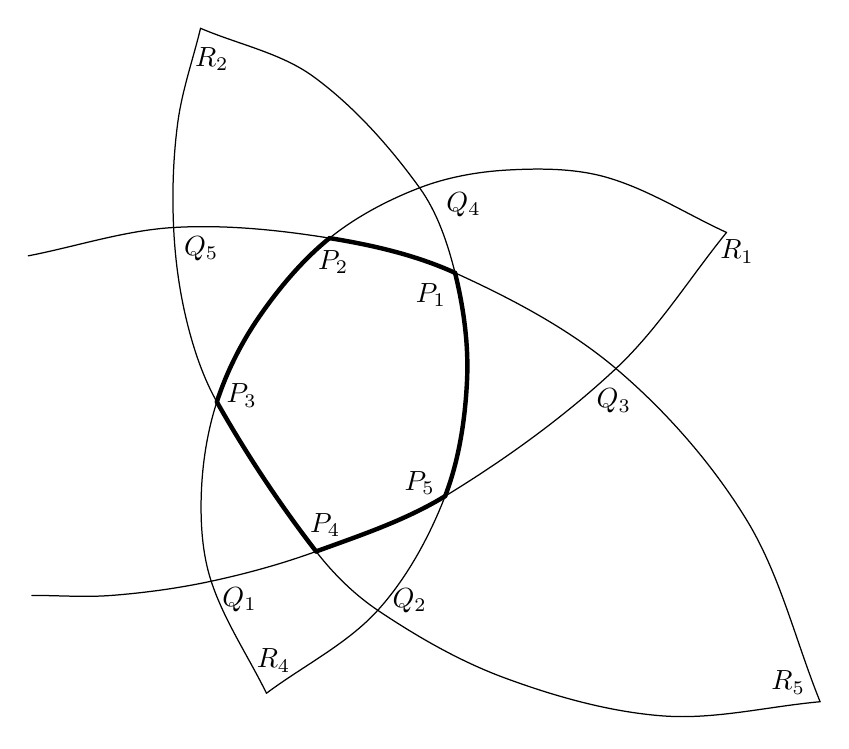
\begin{tikzpicture}[x=.009cm,y=-.009cm,line width=.45pt,line cap=round,line join=round,every node/.style={inner sep=0pt,font=\normalsize}]
\draw (30,336) .. controls (98.333,322.667) and (166.088,300.054) .. (235,296) .. controls (307.754,291.72) and (382.8,299.361) .. (455,311) .. controls (515.133,320.694) and (576.765,334.843) .. (632,360) .. controls (711.431,396.177) and (792.68,438.845) .. (859,495) .. controls (929.68,554.845) and (994.637,629.074) .. (1043,708) .. controls (1090.637,785.741) and (1112.333,879.333) .. (1147,965);
\draw[line width=1.6pt] (455,311) .. controls (515.133,320.694) and (576.765,334.843) .. (632,360);
\draw (35,815) .. controls (72.667,815) and (110.544,817.961) .. (148,815) .. controls (194.877,811.294) and (242.02,804.899) .. (288,795) .. controls (338.02,784.232) and (387.904,770.49) .. (436,753) .. controls (497.904,730.49) and (562.028,709.139) .. (618,675) .. controls (703.028,623.139) and (786.386,563.041) .. (859,495) .. controls (918.72,439.041) and (963,367) .. (1015,303);
\draw[line width=1.6pt] (436,753) .. controls (497.904,730.49) and (562.028,709.139) .. (618,675);
\draw (273,15) .. controls (262.333,59) and (247.038,102.352) .. (241,147) .. controls (234.371,196.019) and (232.728,246.548) .. (235,296) .. controls (237.062,340.882) and (243.206,386.471) .. (254,430) .. controls (263.54,468.471) and (276.537,507.458) .. (296,542) .. controls (337.203,615.124) and (384.695,686.552) .. (436,753) .. controls (460.362,784.552) and (490.015,813.844) .. (523,836) .. controls (578.348,873.177) and (638.442,907.813) .. (701,931) .. controls (772.442,957.48) and (849.434,979.239) .. (925,985) .. controls (998.101,990.573) and (1073,971.667) .. (1147,965);
\draw[line width=1.6pt] (296,542) .. controls (337.203,615.124) and (384.695,686.552) .. (436,753);
\draw (273,15) .. controls (326,37.667) and (386.337,49.75) .. (432,83) .. controls (489.337,124.75) and (540.299,182.245) .. (582,240) .. controls (606.966,274.578) and (621.666,318.357) .. (632,360) .. controls (644,408.357) and (651.209,460.287) .. (649,510) .. controls (646.543,565.287) and (637.872,623.584) .. (618,675) .. controls (595.872,732.251) and (564.027,790.74) .. (523,836) .. controls (480.027,883.406) and (418.333,914) .. (366,953);
\draw[line width=1.6pt] (632,360) .. controls (644,408.357) and (651.209,460.287) .. (649,510) .. controls (646.543,565.287) and (637.872,623.584) .. (618,675);
\draw (1015,303) .. controls (958.333,277) and (904.034,241.758) .. (845,225) .. controls (800.7,212.425) and (751.28,212.36) .. (705,215) .. controls (663.614,217.36) and (620.594,225.18) .. (582,240) .. controls (537.261,257.18) and (492.239,280.979) .. (455,311) .. controls (416.572,341.979) and (383.122,382.143) .. (355,423) .. controls (330.122,459.143) and (309.499,500.335) .. (296,542) .. controls (282.499,583.668) and (275.386,629.178) .. (274,673) .. controls (272.719,713.512) and (275.405,756.668) .. (288,795) .. controls (306.072,850.002) and (340,900.333) .. (366,953);
\draw[line width=1.6pt] (455,311) .. controls (416.572,341.979) and (383.122,382.143) .. (355,423) .. controls (330.122,459.143) and (309.499,500.335) .. (296,542);
\node at (289,58) {$R_2$};
\node at (1030,330) {$R_1$};
\node at (376,907) {$R_4$};
\node at (1102,938) {$R_5$};
\node at (274,326) {$Q_5$};
\node at (644,264) {$Q_4$};
\node at (856,541) {$Q_3$};
\node at (328,821) {$Q_1$};
\node at (568,823) {$Q_2$};
\node at (460,345) {$P_2$};
\node at (598,391) {$P_1$};
\node at (331,533) {$P_3$};
\node at (449,716) {$P_4$};
\node at (582,656) {$P_5$};
\end{tikzpicture}
\end{center}

Dasselbe ist begleitet von zwei weiteren zwei- bez. dreifach gewundenen Fünfecken
$Q_1Q_3Q_5Q_2Q_4$ und $R_1R_4R_2R_5R_3$. Zufolge der Grundeigenschaft des Pentagramma sind
die Winkel dieser beiden letzteren Fünf\SourceLeaf{120}ecke durchweg rechte; sind $s_k$ die Seitenlängen des Pentagramms $P_1\ldots P_5$ (den
Kugelradius gleich 1 gesetzt), so findet man die Seiten der weiteren Fünfecke aus:

\[
\Arc{P_kQ_{k+2}} = \frac{\pi}{2} - s_{k-2}, \qquad \Arc{P_kQ_{k-2}} = \frac{\pi}{2} - s_{k+2},
\]
\[
\Arc{Q_kR_{k+2}} = s_{k+1}, \qquad \Arc{Q_kR_{k-2}} = s_{k-1}.
\]

Unter den Pentagrammen befindet sich insbesondere ein reguläres. Dieses hat die Seitenlänge
$s = \operatorname{arc\,sin}\sqrt{\dfrac{-1+\sqrt{5}}{2}}$ und lässt sich aus dem sphärischen Dreieck der
Winkel $\dfrac{2\pi}{5}, \dfrac{\pi}{2}, \dfrac{\pi}{4}$ durch Reproduction um die Ecke des
ersten Winkels erzeugen.

Die soeben am allgemeinen Pentagramm aufgewiesenen geometrischen Relationen lassen sich
vermöge der Grundformeln des rechtwinkligen sphärischen Dreiecks in Gestalt einer Reihe von
Gleichungen ansetzen; dies ist in den Fragmenten [1] und [3] ausgeführt. ---

Projicirt man das Pentagramm aus dem Kugelmittelpunkt auf eine Tangentialebene mit einem im
Pentagramm gelegenen Berührungspunkt $O$, so entsteht ein ebenes Fünfeck, in dem die fünf
Geraden $\overline{OP_k}$ die Höhen liefern. Das ebene Fünfeck hat somit die beiden,
übrigens für dasselbe bestimmenden, Eigenschaften:

1) die fünf Höhen laufen alle durch einen und denselben Punkt $O$;

2) die einzelne Höhe wird durch $O$ in zwei Stücke getheilt, deren Product für alle Höhen
gleich (und zwar gleich dem Quadrat des Kugelradius) ist.

Die Projectionsebene macht \textsc{Gauss} nun zur Trägerin der complexen Zahlen (cf. Fragment [2])
und wählt insbesondere $O$ als Nullpunkt. Die weiterhin im Fragmente [2] gegebenen
Entwicklungen haben folgenden Sinn. Auf fünf von $O$ ausziehenden Strahlen werden fünf
Punkte $p, p', \ldots, p''''$ willkürlich gewählt; die von \textsc{Gauss} angegebene Verschiebung
dieser Punkte je auf ihren Strahlen bis in die Lagen $q, q', \ldots, q''''$ liefert alsdann
in diesen letzten Punkten die Ecken eines Pentagramms unserer Art. ---

Ist $M$ der Kugelmittelpunkt, so lässt sich durch die fünf nach den Pentagrammecken $P_k$
ziehenden Strahlen $\overline{MP_k}$ ein eindeutig bestimmter Kegel zweiten Grades legen.
Der letztere und namentlich die Trans\SourceLeaf{121}formation desselben auf seine Hauptaxen spielen in den weiteren \textsc{Gauss}'schen Entwicklungen
eine grundlegende Rolle. Die cubische Gleichung dieser Hauptaxentransformation, welche
allein vom Product der fünf Tangenten der Pentagrammseiten abhängt, wird auch nach ihrer
numerischen Seite in [5] behandelt. Will man übrigens die zahlreichen Relationen der
Fragmente [5] und [6] beweisen, so knüpft man am besten an die wohlbekannten neueren
Grundformeln für die Hauptaxentransformation eines Kegels an. Bei dem von \textsc{Gauss} zunächst
ausgewählten Coordinatensystem $x, y, z$ kann man aus jenen Grundformeln die Gleichungen
der genannten Fragmente fast ohne Rechnung ableiten. ---

Die Entwicklungen unter [7] und [8], welche das Datum 1843 April 20 tragen, begründen die
Beziehung des Pentagramms zur Fünftheilung der elliptischen Functionen. Es ist
unzweifelhaft, dass \textsc{Gauss} diese Beziehung auf Anregung von \textsc{Jacobis} Abhandlung Ȇber die
Anwendung der elliptischen Transcendenten auf ein bekanntes Problem der
Elementargeometrie«\footnote{\textsc{Crelles} Journal Bd. 3 (1828).} erkannt hat. \textsc{Jacobi} studirt
daselbst Fünfecke, deren einzelnes einem Kreise eingeschrieben und zugleich einem zweiten
Kreise umschrieben ist, und weist deren Beziehung zu den elliptischen Functionen auf.

Um den Übergang vom Pentagramm zum \textsc{Jacobi}schen Fünfeck zu bewerkstelligen, projicire man
ersteres vom Kugelmittelpunkt auf diejenige Tangentialebene der Kugel, deren
Berührungspunkt der Durchschnittspunkt der Kugel mit der Kegelaxe ist. Der Kegel wird von
dieser Projectionsebene in einer Ellipse geschnitten, welcher das projicirte Pentagramm
eingeschrieben ist. Die hierneben in der Figur angedeutete affine Transformation liefert in
$P_1'P_2'\,..\,P_5'$ ein \textsc{Jacobi}sches Fünfeck.

\begin{center}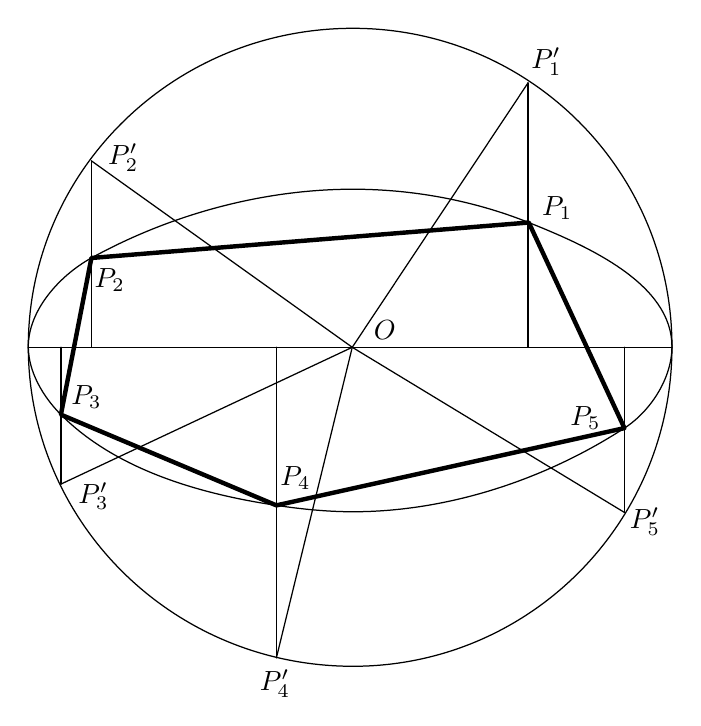
\begin{tikzpicture}[x=.009cm,y=-.009cm,line width=.45pt,line cap=round,line join=round,every node/.style={inner sep=0pt,font=\normalsize}]
\draw (41,480) .. controls (41,232) and (246,31) .. (499,31) .. controls (748,31) and (949,232) .. (949,480) .. controls (949,729) and (748,931) .. (499,931) .. controls (246,931) and (41,729) .. cycle;
\draw (41,480) .. controls (41,428.851) and (85.182,379.65) .. (130,355) .. controls (241.436,293.71) and (371.821,258) .. (499,258) .. controls (583.138,258) and (668.88,273.752) .. (747,305) .. controls (829.716,338.086) and (949,390.913) .. (949,480) .. controls (949,524.365) and (919.197,570.822) .. (882,595) .. controls (769.994,667.804) and (632.589,713) .. (499,713) .. controls (462.875,713) and (426.725,709.359) .. (391,704) .. controls (282.267,687.69) and (164.746,653.746) .. (87,576) .. controls (61.909,550.909) and (41,515.484) .. (41,480);
\draw (41,481)--(949,481);
\draw (498,481)--(746,108);
\draw (746,108)--(746,481);
\draw (498,481)--(130,218);
\draw (130,218)--(130,481);
\draw (498,481)--(87,674);
\draw (87,674)--(87,481);
\draw (498,481)--(391,919);
\draw (391,919)--(391,481);
\draw (498,481)--(882,714);
\draw (882,714)--(882,481);
\draw[line width=1.6pt] (747,305)--(130,355)--(87,576)--(391,704)--(882,595)--cycle;
\node at (772,78) {$P_1'$};
\node at (175,213) {$P_2'$};
\node at (133,691) {$P_3'$};
\node at (389,956) {$P_4'$};
\node at (911,727) {$P_5'$};
\node at (787,284) {$P_1$};
\node at (156,386) {$P_2$};
\node at (123,551) {$P_3$};
\node at (418,665) {$P_4$};
\node at (827,581) {$P_5$};
\node at (544,457) {$O$};
\end{tikzpicture}
\end{center}

Die Richtigkeit dieser Angaben geht aus der Übereinstimmung der \textsc{Gauss}'schen Formeln in [7]
und [8] mit den von \textsc{Jacobi} a.\,a.\,O. entwickelten Gleichungen hervor. Zum Beweise der
\textsc{Gauss}'schen Relationen kann man so verfahren:

Benutzt man in der Projectionsebene die Hauptaxen der Ellipse als Axen $x, y$ und setzt den
Kugelradius gleich 1, so liegt der Kugelmittelpunkt senkrecht zur Ebene unter $O$ in der
Entfernung 1. Die Grundeigenschaft des Pentagramms, dass nämlich
$\HistAngle P_{k-1}MP_{k+1} = \dfrac{\pi}{2}$ ist, liefert die fünf Gleichungen:

\[
x_{k-1}x_{k+1} + y_{k-1}y_{k+1} + 1 = 0,\tag{1}
\]
\SourceLeaf{122}wenn $x_k, y_k$ die Coordinaten von $P_k$ sind. Das einzelne Paar $x_k, y_k$ kommt in zwei
Gleichungen vor, durch deren Auflösung man findet:

\[
x_k = \dfrac{y_{k+2}-y_{k-2}}{x_{k+2}y_{k-2}-x_{k-2}y_{k+2}}, \qquad
y_k = \dfrac{x_{k-2}-x_{k+2}}{x_{k+2}y_{k-2}-x_{k-2}y_{k+2}}.\tag{2}
\]

Ist nun, wie bei \textsc{Gauss}, $\varphi_k$ die excentrische Anomalie von $P_k$, so sind die
Coordinaten von $P_k'$ offenbar $\cos\varphi_k, \sin\varphi_k$, und man findet als
Coordinaten von $P_k$:

\[
x_k = \sqrt{\dfrac{-G}{G'}}\cos\varphi_k, \qquad y_k = \sqrt{\dfrac{-G}{G''}}\sin\varphi_k,
\]

$G, G'$ und $G''$ im Sinne von \textsc{Gauss} gebraucht. Durch Eintragung dieser Werthe in die
Gleichungen (2) ergeben sich die ersten unter [7] angegebenen \textsc{Gauss}'schen Gleichungen:

\[
\dfrac{\cos\frac{1}{2}(\varphi_{k+2}+\varphi_{k-2})}{\cos\frac{1}{2}(\varphi_{k+2}-\varphi_{k-2})}
= \dfrac{G}{G'}\cos\varphi_k, \qquad
\dfrac{\sin\frac{1}{2}(\varphi_{k+2}+\varphi_{k-2})}{\cos\frac{1}{2}(\varphi_{k+2}-\varphi_{k-2})}
= \dfrac{G}{G''}\sin\varphi_k.
\]

Eliminirt man hier $\varphi_k$ und schreibt hernach $k$ statt $k+2$, so folgt:

\[
G'^2\cos^2\tfrac{1}{2}(\varphi_k+\varphi_{k+1}) + G''^2\sin^2\tfrac{1}{2}(\varphi_k+\varphi_{k+1})
= G^2\cos^2\tfrac{1}{2}(\varphi_k-\varphi_{k+1}),
\]
\[
G^2\cos(\varphi_{k+1}-\varphi_k) + (G''^2-G'^2)\cos\varphi_{k+1}+\varphi_k) = G'^2+G''^2-G^2.
\]

Durch Entwicklung der Cosinus und Einführung der Coordinaten der Punkte $P_k$ folgt weiter:

\[
(G^2-G'^2+G''^2)G'x_kx_{k+1} + (G^2+G'^2-G''^2)G''y_ky_{k+1} +
(-G^2+G'^2+G''^2)G = 0.\tag{3}
\]

Nun sind die $G, G', G''$ Wurzeln der Gleichung

\[
G(2G-1)^2 = \alpha\beta\gamma\delta\varepsilon(G-1).
\]

Es ergibt sich demnach für das Absolutglied der letzten Gleichung:

\[
(G^2+G'^2+G''^2-2G^2)G = \left(\dfrac{1+\alpha\beta\gamma\delta\varepsilon}{2} - 2G^2\right)G
= \dfrac{\alpha\beta\gamma\delta\varepsilon}{2}\cdot\dfrac{1}{2G-1},
\]

und man findet analoge Ausdrücke für die Coefficienten der beiden ersten Glieder der
Gleichung (3), so dass jene Gleichung übergeht in:

\[
\dfrac{x_kx_{k+1}}{2G'-1} + \dfrac{y_ky_{k+1}}{2G''-1} + \dfrac{1}{2G-1} = 0.\tag{4}
\]

Indem man diese Gleichung ebenso behandelt wie (1), ergeben sich die weiteren im Fragmente
[7] zusammengestellten Relationen.

Die vorstehenden Angaben über die Beziehung zwischen \textsc{Gauss} und \textsc{Jacobi} werden in ein neues
Licht durch die Bemerkung gesetzt, dass jedes beliebige gewöhnliche Fünfeck ohne
einspringende Winkel collinear in ein \textsc{Jacobi}sches und also auch in ein \textsc{Gauss}'sches
Pentagramm transformirt werden kann. Dem gegebenen Fünfeck lässt sich nämlich eine
bestimmte Ellipse einschreiben und ein gleichfalls bestimmter Kegelschnitt umschreiben. Man
hat nur nöthig, dieses Kegelschnittpaar in ein Kreispaar collinear zu überführen, was nach
heute wohlbekannten Methoden keine Schwierigkeit hat.

Diese Bemerkung ist auch für die Entwicklungen in den Fragmenten [9] bis [11] von
Wichtigkeit. \textsc{Gauss} construirt hier zunächst durch fortgesetztes Diagonalenziehen bez.
Seitenverlängern eine nach beiden
\SourceLeaf{123}Seiten hin unendliche Kette von Fünfecken und erkennt, dass dieses Netz einander umschliessender Fünfecke

\begin{center}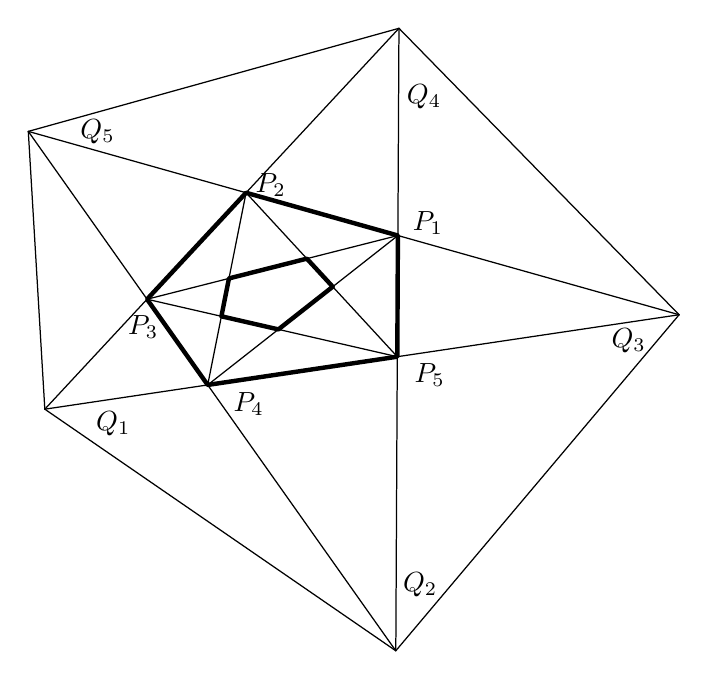
\begin{tikzpicture}[x=.01cm,y=-.01cm,line width=.45pt,line cap=round,line join=round,every node/.style={inner sep=0pt,font=\normalsize}]
\coordinate (Q5) at (392,534);
\coordinate (Q4) at (863,403);
\coordinate (Q3) at (1219,767);
\coordinate (Q2) at (859,1194);
\coordinate (Q1) at (413,887);
\coordinate (P2) at (668.717,611.962);
\coordinate (P1) at (861.668,666.325);
\coordinate (P5) at (860.89,820.317);
\coordinate (P4) at (619.971,856.186);
\coordinate (P3) at (542.909,747.276);
\draw (Q5)--(Q4);
\draw (Q4)--(Q3);
\draw (Q3)--(Q2);
\draw (Q2)--(Q1);
\draw (Q1)--(Q5);
\draw (Q5)--(Q3);
\draw (Q3)--(Q1);
\draw (Q1)--(Q4);
\draw (Q4)--(Q2);
\draw (Q2)--(Q5);
\draw (P2)--(P5);
\draw (P5)--(P3);
\draw (P3)--(P1);
\draw (P1)--(P4);
\draw (P4)--(P2);
\draw[line width=1.6pt] (P2)--(P1)--(P5)--(P4)--(P3)--cycle;
\draw[line width=1.6pt] (646.984,720.845)--(745.96,695.71)--(778.856,731.376)--(709.811,785.614)--(637.377,768.975)--cycle;
\node at (480,534) {$Q_5$};
\node at (895,490) {$Q_4$};
\node at (1155,800) {$Q_3$};
\node at (890,1110) {$Q_2$};
\node at (500,905) {$Q_1$};
\node at (700,602) {$P_2$};
\node at (900,650) {$P_1$};
\node at (902,844) {$P_5$};
\node at (672,880) {$P_4$};
\node at (538,783) {$P_3$};
\end{tikzpicture}
\end{center}

durch die Collineation:

\[
x' = \dfrac{2\,G-1}{2\,G'-1}\,x, \qquad y' = \dfrac{2\,G-1}{2\,G''-1}\,y\tag{5}
\]

in sich transformirt wird. Zur Erläuterung vergl. man die beigefügte Figur; \textsc{Gauss} hat selber Zeichnungen dieser Art angefertigt, in denen die Fünfecknetze noch viel weiter fortgesetzt sind. Die in (5) rechter Hand stehenden Coefficienten sind die »Exponenten« oder »Coefficienten der Verjüngung«, welche in [9] und [10] auftreten. Es liegt sehr nahe, das hier vorliegende Sachverhältniss im Sinne der modernen Theorie der discontinuirlichen Substitutionsgruppen aufzufassen. Der Nullpunkt $O$ erscheint dabei als der innere Grenzpunkt des Pentagrammnetzes und ist einer der drei Grenzpunkte der aus (5) entspringenden cyclischen Collineationsgruppe.

Zufolge der voraufgesandten Bemerkung findet die gleiche Sachlage bei jedem Fünfeck mit einspringenden Winkeln statt. Diese Verhältnisse sind in der neueren Litteratur wohlbekannt.

Die Richtigkeit der \textsc{Gauss}'schen Angaben kann man so bestätigen: Das an $P_1P_2\,..\,P_5$ sich zunächst anschliessende äussere Fünfeck $Q_1Q_2\,..\,Q_5$ ist dasselbe, welches aus dem so benannten sphärischen Fünfeck bei der Projection entsteht. Hat $Q_k$ die Coordinaten $x'_k$, $y'_k$, so gelten, da $\HistAngle\,Q_kMP_{k+1} = \dfrac{\pi}{2}$ ist, die fünf Gleichungen:

\[
x'_k x_{k+1} + y'_k y_{k+1} + 1 = 0.
\]

Der Vergleich mit den fünf Gleichungen (4) lässt für alle Indices $k$ die Formeln (5) als richtig erscheinen.

\SourceLeaf{124}
Dass \textsc{Gauss} den projectiven Charakter seiner zuletzt besprochenen Entwicklungen gekannt hat, macht namentlich das Fragment [11] wahrscheinlich. \textsc{Gauss} wendet hier die Grundsätze von \textsc{Moebius}' barycentrischem Calcul auf die Figur des geradlinigen Pentagramms an; man wird die \textsc{Gauss}'schen Formeln im Sinne dieses Calculs ohne Mühe verstehen. Dem projectiven Charakter des letzteren entsprechend wird hier an ein beliebiges Fünfeck angeknüpft. Zufolge eines Briefes an \textsc{Schumacher} vom 15. Mai 1843 hat \textsc{Gauss} erst am 14. Mai dieses Jahres das (1827 erschienene) \textsc{Moebius}'sche Werk über den barycentrischen Calcul kennen gelernt und zwar vermuthlich aus Anlass der Aufgabe, den Mittelpunkt eines durch fünf Punkte gegebenen Kegelschnitts durch Construction zu finden. Für die speciellen Fünfecknetze, auf welche sich die Formeln der Fragmente [5] bis [10] beziehen, würde jene Aufgabe identisch sein mit dem Problem, den inneren Grenzpunkt des einzelnen Netzes zu construiren. Übrigens stammt die Entwicklung der Fragmente [7] und [8] aus dem April 1843, und diejenige des Fragmentes [11] schliesst sich (wahrscheinlich unmittelbar) an den 14. Mai 1843. Hiernach wird man annehmen dürfen, dass die in [9] und [10] aufgenommenen Untersuchungen in den zwischen beiden Daten gelegenen Wochen ausgeführt sind.

\hfill\textsc{Fricke}.

\noindent\hrulefill\par

\end{document}
